\chapter{Objet}

Ce document a pour but de présenter l'architecture technique de ce projet. Le but de ce projet est de développer un outil de protection et de gestion des licences.

\chapter{Documents de référence}

Documents de spécification :

\begin{itemize}
    \item Spécification Technique des Besoins
    \item Fiches techniques :
	\begin{itemize}
	    \item Injection de code dans un PE
	    \item Génération de licence
	    \item Signature
	    \item Obfuscation de code
	    \item Sécurisation des bases de données
	\end{itemize}
\end{itemize}

\chapter{Terminologie}

\chapter{Configuration requise}

Les éléments matériels nécessaire au développement de cet outil sont :

\begin{itemize}
    \item Un serveur
\end{itemize}

\chapter{Architecture statique}
Afin de réaliser ce projet nous avons choisit de mettre en place l'infrastructure suivante:

\begin{description}
	\item[\textbf{Un serveur web}:]
				C'est ce serveur qui présentera l'interface aux utilisateur et  
				\begin{itemize}
					\item Permettra à un client de se créer un compte, demander et 
								télécharger l'outil de generation de licence.
					\item Permettra à un administrateur d'accorder et de gérer les licences. 
				\end{itemize}
	\item[\textbf{Un logiciel d'activation}:] 
				Sera executé sur la machine de l'utilisateur
				afin de lui permettre de générer une licence. Pour cela il échangera avec
				le serveur des informations sur le matériel physique de la machine, ce 
				qui permettra à ce dernier de générer le fichier de licence.
	\item[\textbf{Outil de Validation}:]
				Outil permettant de vérifier la validité d'une licence, cette outil
				pourra prendre les formes suivantes: 
				\begin{itemize}
				\item Une bibilothèque de fonctions qui permettra à un developpeur d'inclure
							dans son code les fonctions de vérification de licence. 
				\item Un programme permettant de greffer directement les fonctions de vérification
							sur un exécutable. 
				\end{itemize}
\end{description}

L'architecture générale de ce projet peut être représenter via 
le schéma n°\ref{fig:fig1}\newline

\begin{figure}[h!]
	\centering
	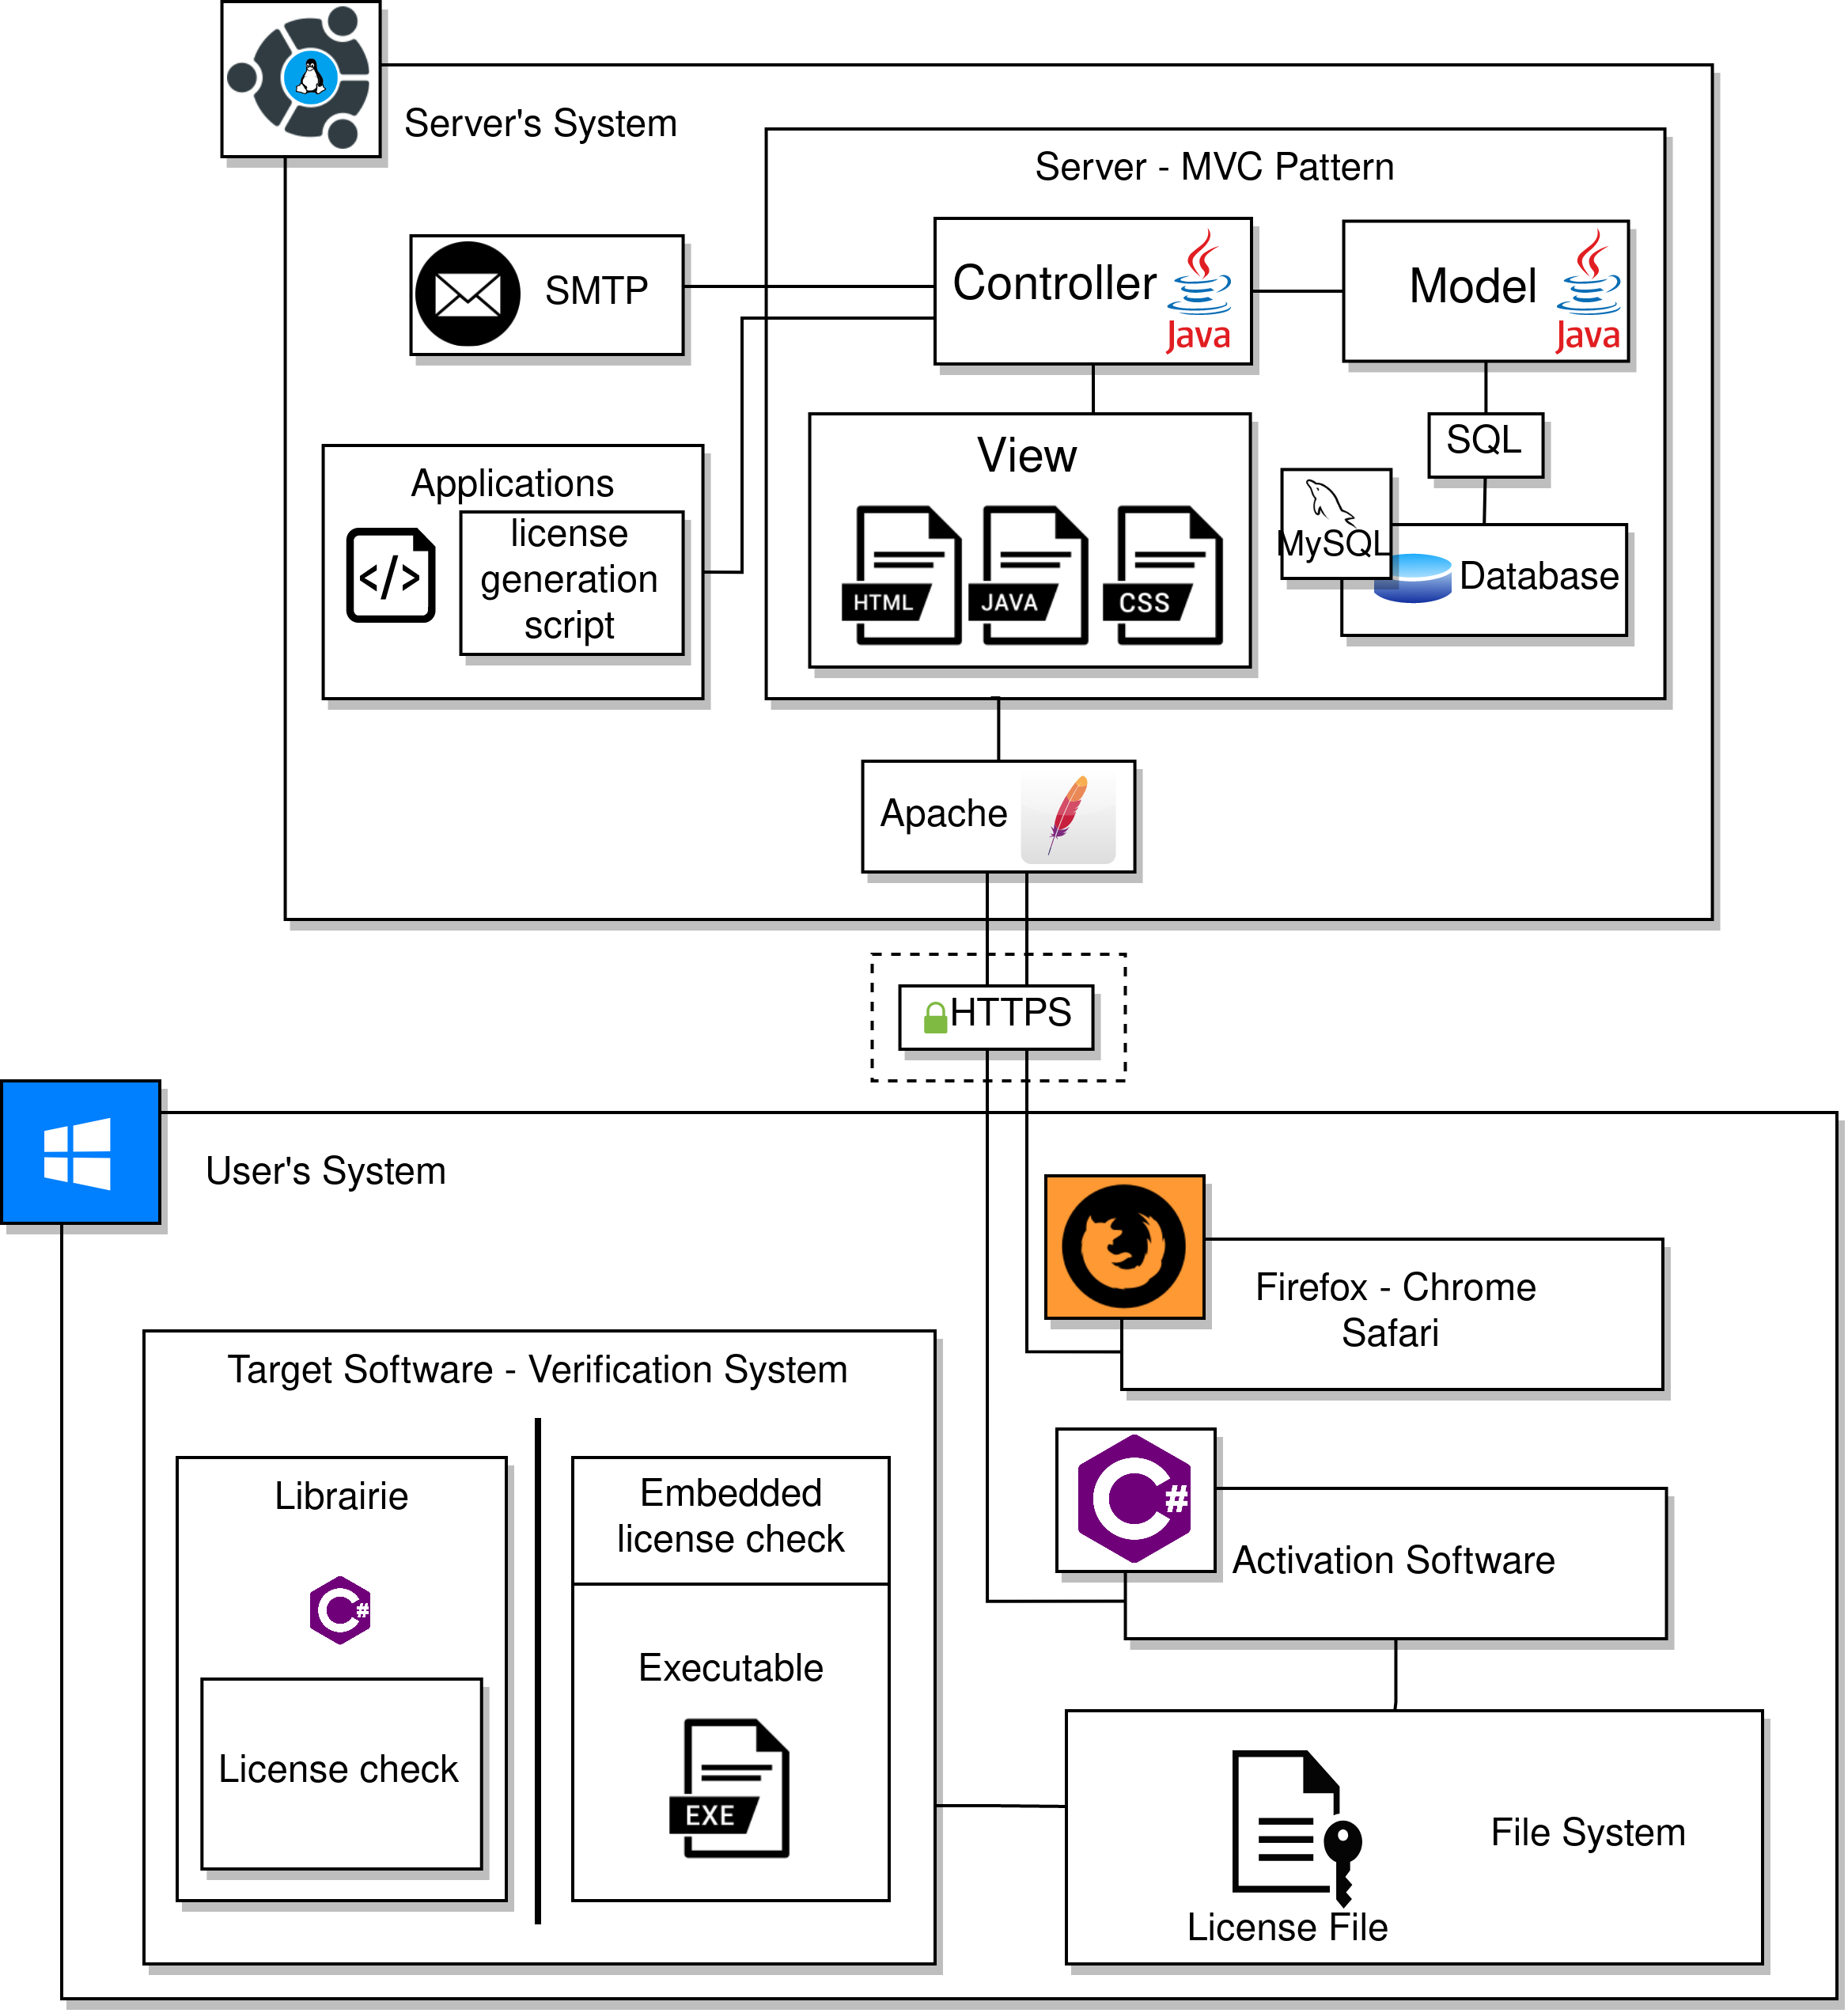
\includegraphics{../png/DAT_general.png}
	\caption{Schéma d'architecture générale}
	\label{fig:fig1}
\end{figure}
\newpage

\section{Constituant «application»}

\subsection{Description}

\begin{description}
	\item[\textbf{Rôle}:]
				Le but du serveur est de fournir l'interface principale, programmé 
				en HTML, CSS et JS aux utilisateurs, de stocker dans sa base de donnée
				les informations nécessaires à la génération de licence et enfin de générer 
				les licences.
	%\item[\textbf{Propriétés et attributs de caractérisation}:]
	\item[\textbf{Services offerts}:]
				API Rest \cite{REST} permettant à au client d'envoyer les informations
				nécéssaires à la génération de la licence (voir \ref{fig:fig2})				
	\item[\textbf{Dépendances}:]
				Dépend du module de Base de données.
	\item[\textbf{Langages}:]
				HTML, CSS, JS, PHP, SQL, Bash, C 
	\item[\textbf{Procédé de développement}:]
				Utilisation du pattern design MVC (Model Vue Controler) avec le framework codeIgniter et respect des
                conventions Material Design \cite{Material}.

	\item[\textbf{Taille et complexité}:]
				Taille importante et complexité élévé.
\end{description}

\subsection{Justifications techniques.}
Utilisation de la pile LAMP (Linux, Apache, MySQL, PHP) car beaucoup de 
support et de documentation \cite{LAMP}, Il y a possibilité d'automatiser 
le deploiement de la solution via un script d'installation. \newline
Le serveur utilisera un script permettant de générer une licence pour un 
utilisateur en prenant en paramètre l'id du logiciel pour lequelle on doit 
générer la licence, un hash des informations hardware du client, et les
attributs de la licence (nombre d'essais, période de validité) et renverra
le fichier de licence. Le script utilisera les fonctions suivantes:
\begin{minted}{c}

// Récupère les droits d'une licence à partir d'un fichier de
// licence, renseigné par son chemin.
char *hashWithSHA256(const char *string);

// Génère une signature de dataToSign à partir de la clé privé asymétrique 
//  privateKey. 
char *generateSignature(const char *dataToSign, const char *privateKey);
  
// Encode une chaîne de caractères en base64
char *encodeBase64(const char *string);

\end{minted}

\begin{figure}[hp!]
	\caption{API rest}
	\definecolor{getColor}{rgb}{0.28, 0.8, 0.56}
\definecolor{postColor}{rgb}{0.38, 0.68, 0.99}

\usemintedstyle{monokai}
\definecolor{bg}{HTML}{282828} % from https://github.com/kevinsawicki/monokai

\begin{tcolorbox}[title=RestFull API]

	\begin{tcbitemize}[%
    raster columns=7, 
    raster rows=2, 
    raster equal height=rows,
    ]

		% Row I
		\tcbitem[myhbox={}{},
			colback=getColor,colupper=white, 
			fontupper=\sffamily\bfseries\normalsize]	GET
		\tcbitem[raster multicolumn=6, myhbox={}{},
						 fontupper=\ttfamily\bfseries\normalsize] /api/v1/Software/getSoftwareList

		% Row II
		\tcbitem[raster multicolumn=5, myhbox={}{}, 
						 frame hidden, interior hidden] \textbf{Parameters:} 

		\tcbitem[raster multicolumn=2, colback=white, 
						 colupper=black, myhbox={}{}] No parameters 

		% Row III
		\tcbitem[raster multicolumn=3, myhbox={}{}, 
						 frame hidden, interior hidden] \textbf{Response:} 

		\tcbitem[raster multicolumn=2, myhbox={}{}, 
						 frame hidden, interior hidden] \emph{content type}

		\tcbitem[raster multicolumn=2, colback=white, 
						 colupper=black, myhbox={}{}] application/json

		% Row IV
		\tcbitem[raster multicolumn=7, myhbox={}{}]
		\begin{tcbitemize}[raster columns=7, 
											 raster rows=2]
				
			\tcbitem[raster multirow=1, myhbox={}{},
							 fontupper=\sffamily\bfseries\normalsize,
							 frame hidden, interior hidden] 200

			\tcbitem[raster multirow=1, raster multicolumn=6, myhbox={}{}, colback=bg] 
					\begin{minted}[bgcolor=bg, breaklines, breakautoindent=true]{json}
[{
	"SoftwareId" : 0,
	"SoftwareName" : "Logiciel de Gestion de Paye",
	"SoftwareDesc" : "Permet de gérer les payes de vos employés"
}]
				\end{minted}
			
			\tcbitem[raster multirow=1, myhbox={}{},
							 fontupper=\sffamily\bfseries\normalsize,
							 frame hidden, interior hidden] 404

			\tcbitem[raster multirow=1, raster multicolumn=6, myhbox={}{}] Not Found

		\end{tcbitemize}

		% Row V			
		\tcbitem[myhbox={}{},
			colback=postColor,colupper=white, 
			fontupper=\sffamily\bfseries\normalsize]	POST
		\tcbitem[raster multicolumn=6, myhbox={}{},
						 fontupper=\ttfamily\bfseries\normalsize] /api/v1/Licence/requestLicence

	% Row III
	\tcbitem[raster multicolumn=3, myhbox={}{}, 
					 frame hidden, interior hidden] \textbf{Parameters:} 

	\tcbitem[raster multicolumn=2, myhbox={}{}, 
					 frame hidden, interior hidden] \emph{content type}

	\tcbitem[raster multicolumn=2, colback=white, 
					 colupper=black, myhbox={}{}] application/json

	\tcbitem[raster multicolumn=7, myhbox={}{}, colback=bg] 
					\begin{minted}[bgcolor=bg, breaklines, breakautoindent=true]{json}
[{
	"UserMail" : "prenom.nom@mail.com",
	"UserPassword" : "123456seven",
	"SoftwareId" : 0,
	"HardwareHash" : "2e41d4a7-8be7-40ef-8b29-e77aadee37cb"
}]
				\end{minted}
		
	% Row II
	\tcbitem[raster multicolumn=7, myhbox={}{}, 
					 frame hidden, interior hidden] \textbf{Response:} 

	% Row IV
	\tcbitem[raster multicolumn=7, myhbox={}{}]
	\begin{tcbitemize}[raster columns=7, 
										 raster rows=2]
			
		\tcbitem[raster multirow=1, myhbox={}{},
						 fontupper=\sffamily\bfseries\normalsize,
						 frame hidden, interior hidden] 200

		\tcbitem[raster multirow=1, raster multicolumn=6, myhbox={}{}] LicenceFile.key 

		\tcbitem[raster multirow=1, myhbox={}{},
						 fontupper=\sffamily\bfseries\normalsize,
						 frame hidden, interior hidden] 404

		\tcbitem[raster multirow=1, raster multicolumn=6, myhbox={}{}] Not Found

		\end{tcbitemize}

	\end{tcbitemize}
\end{tcolorbox}

	\label{fig:fig2}
\end{figure}
\newpage

\section{Constituant «Base de données»}

\begin{figure}[h!]
	\centering
	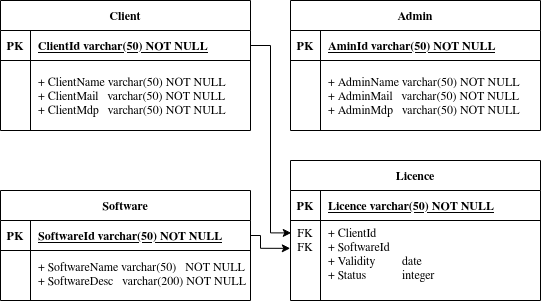
\includegraphics[width=\textwidth - 2cm]{../png/SQL_table.png}
	\caption{Diagramme UML des Tables de la BDD}
	\label{fig:fig2}
\end{figure}

\subsection{Description}
\begin{description}
	\item[\textbf{Rôle}:]
		Le but de ce module est de permettre de stocker les informations relatives aux
		clients, administrateurs et aux licences. 
%	\item[\textbf{Propriétés et attributs de caractérisation}:]
	\item[\textbf{Services offerts}:]
		Fonctions SQL permettant de creer / modifier / supprimer / consulter les 
	  informations relatives aux clients, administrateurs et licences.
	\item[\textbf{Dépendances}:]
		Pas de dépendances.		
	\item[\textbf{Languages}:]
		MySQL.
	\item[\textbf{Procédé de développement}:]
	  Porter une attention partculière à la sécurisation des données, via
	  du chiffrement et à se proteger des attaques du type «injections SQL». 
	\item[\textbf{Taille et complexité}:]
		Taille faible et complexité faible. 
\end{description}

\subsection{API PHP/SQL}
Nous utiliserons MySQL avec PHP pour interagir avec notre base de données (partie model) depuis la plateforme Web.

Une API des fonctions PHP utilisées est disponible en annexe (voir section \ref{section:php}).

% \subsection{Justifications techniques.}

\section{Constituant «Logiciel d'activation»}
\subsection{Description}
\begin{description}
	\item[\textbf{Rôle}:]
		Récuperer les informations matériels sur la machine d'un utilisateur, puis 
		se connecter au serveur afin de générer le fichier de licence.
%	\item[\textbf{Propriétés et attributs de caractérisation}:]
	\item[\textbf{Services offerts}:] 
		n'offre aucun service.
	\item[\textbf{Dépendances}:]
		Dépend du Module Serveur.
	\item[\textbf{Languages}:]
		C\#.
	\item[\textbf{Procédé de développement}:]
		Respect d'une charte de code. (Voir Chapitre \ref{chap:Annexe})
	\item[\textbf{Taille et complexité}:]
		Taille faible et complexité faible. 
\end{description}

\subsection{Justifications techniques.}

\section{Constituant «Système de véfication - Librairie»}
\subsection{Description}
\begin{description}
	\item[\textbf{Rôle}:]
		Fournir une API pour des programmes en C\# afin de 
		permettre à un developpeur de vérifier une licence dans son code.
        Cependant le code de la bibliothèque ne sera pas en C\# mais en 
        C car celui-ci est plus facile à obfusquer. 
%	\item[\textbf{Propriétés et attributs de caractérisation}:]

	\newpage

	\item[\textbf{Services offerts}:]
		Ce module propose une API dont des fonctions sont les suivantes:
		\begin{minted}{csharp}
/*
 * Récupère l'identifiant de la carte réseau.
 */
public String getNetworkAdapterNo();

/*
 * Récupère le numéro de série du BIOS.
 */
public String getBIOSSerialNo();

/*
 * Récupère le numéro de série du disque.
 */
public String getDiskSerialNo();

/*
 * Récupère les droits d'une licence à partir d'un fichier de
 * licence, renseigné par son chemin.
 */
public String getRights(String pathToLicenseFile);

/*
 * Vérifie la signature à partir des informations du système,
 * de l'identifiant du logiciel, situé dans le programme, des
 * droits, obtenus à partir du fichier de licence.
 */
public int verifySignature(String pathToLicenseFile);

/*
 * Génère un hashé à partir d'une chaîne de caractères donné
 * en entrée, en utilisant l'algorithme SHA-256.
 */
public String hashWithSHA256(String s);

/*
 * Décode une chaîne de caractères encodée en base64.
 */
public String decodeBase64(String s);
			\end{minted}

	\item[\textbf{Dépendances}:]
		Dépend d'un fichier de licence.	
	\item[\textbf{Languages}:]
		C, C++, C\#
	\item[\textbf{Procédé de développement}:]
		Respect d'un charte de code. (Voir Chapitre \ref{chap:Annexe})
	\item[\textbf{Taille et complexité}:]
		Taille importante et complexité relative.
\end{description}

\subsection{Justifications techniques.}
Dans un premier temps, les fonctions de l'API pourront être implémentées en utilisant des bibliothèques systèmes comme par exemple pour les informations hardware la 
classe \verb:System.Management:, ou bien la classe \verb:System.Security.Cryptography: 
pour le hash avec SHA-256.\newline

Dans un second temps, nous devrons implanter au maximum les fonctions nous-mêmes et 
les optimisés dans le but de pouvoir intégrer ces fonctions directement dans un 
exécutable (greffe dans un PE) sans pour autant alourdir ou ralentir l'éxécution de 
l'application. \newline

C'est aussi dans un but pédagogique nous avons choisit d'implémenter nous même le système cryptographique de signature, le schéma de signature retenu est ElGamal \cite{ElGamal}.

\section{Constituant «Système de véfication - Greffe»}
\subsection{Description}
\begin{description}
	\item[\textbf{Rôle}:]
			Outil permettant d'ajouter les fonctions de vérification directement à un
			executable, afin de décharger le developpeur de la necessité de vérifier 
			la licence dans son code.
%	\item[\textbf{Propriétés et attributs de caractérisation}:]
	\item[\textbf{Services offerts}:]
		n'offre auxun service.
	\item[\textbf{Dépendances}:]
		Dépend de la bibliothèque de vérification.
	\item[\textbf{Languages}:]
		C, C\#, Python, Bash 
	\item[\textbf{Procédé de développement}:]
		Respect d'un charte de code. (Voir Chapitre \ref{chap:Annexe}) 
	\item[\textbf{Taille et complexité}:]
		Taille faible et complexité élevé.
\end{description}

% \subsection{Justifications techniques.}

\chapter{Annexe}
\label{chap:Annexe}

\section{Formatage du code}
Les accolades sont positionnées en fin et début de fonction ou de bloc en 
respectant les conventions adoptées dans les environnements Visual Studio 
mais aussi www.gnu.org. Ce formatage permet de rendre le code plus aéré, 
et ainsi faciliter la relecture.

\begin{minted}{c}
static char *concat(char *s1, char *s2)
{
    ...
}
\end{minted}

Le code sera tabulé par bloc comme dans l'exemple suivant:
\begin{minted}{c}
void foo(int x)
{
    int res = 0;
    for (int i = 0; i < x; ++i)
    {
        res += i * x;
    }
    printf("res : %d\n", res);
}
\end{minted}

De plus les recommandations suivantes seront respectés:
\begin{itemize}
	\item Une seule instruction par ligne
	\item Une seule déclaration par ligne
	\item Une tabulation sera transformé en quatre espaces.	
	\item La longueur maximale d'une ligne est de 80 charactères.
        \item La définition des variables se fait au debut d'une fonction avant
              toutes autres instructions. 
\end{itemize}

Enfin les opérandes utilisés pour les opérations \mintinline{c}{&&} et \mintinline{c}{||}
seront entourés de parenthèses afin d'éviter les ambiguités:
\begin{minted}{c}
if ((x != 0) && (isValid(y) || y == 5))
{
    ...
}
\end{minted}

\section{Sortie de fonctions}

Un seul \mintinline{c}{return} par fonction afin de
\begin{itemize}
	\item Faciliter la trace de la sortie
	\item Le placement de break points lors du debug
	\item Faciliter l’analyse de la fonction
\end{itemize}

Les \mintinline{c}{goto} sont interdit.

\section{Commentaires}
Les commentaires ne doivent pas qu’uniquement formuler en texte ce qui est traduit 
en dans le langage de programmation (qui se doit d'être lisible) : \newline 
Ils apportent une réelle plus-value dans la compréhension du programme ou doivent
attirer l’attention du mainteneur sur certains choix réalisés. Les commentaires seront 
rédigés en anglais. \newline
Un commentaire doit être sur une seule ligne (ne peut pas être sur la même ligne 
que du code).
 
\section{Nommages}
Pour la définition d'un type, d'une struct ou d'une classe la notation 'PascalCase'
sera utilisé: 
\begin{minted}{c}
typedef struct 
{
    ...
}
SuperComplexDataType;
\end{minted}

Pour les variables et les fonctions les noms devront être significatifs et 
pertinents.\newline
Ils sont constitués uniquement des caractères non accentués suivants: 
[a-z], [A-Z], [0-9]\newline
Avec les restrictions suivantes :
\begin{itemize}
	\item Le nom ne doit pas commencer par un chiffre
	\item Le nom ne peut pas avoir de caractères "underscore"
	\item Les noms doivent être en 'camelCase', en Anglais
	\item Les noms ne peuvent pas commencer par des majuscules exception faite
          des acronymes (voir plus bas).
\end{itemize}
Les noms doivent être homogènes pour un domaine fonctionnel donné. Par exemple, 
toutes les fonctions relatives à la gestion de la mémoire dans une API peuvent 
être du type: \newline 
APIMemoryOpen(), APIMemoryClose(), APIMemorySet(...)



\section{API PHP}
\label{section:php}
\inputminted{php}{api.php}